\chapter{Introduction}
\label{introduction}

\section{A Brief History of Galaxy Evolution}
{\bf MRB says: I would think of these first three 
sections as close to just a single section. I might 
also suggest the opening section be "Questions in 
galaxy evolution." You could have a paragraph or two
on the thumbnail history --- Herschel to Slipher and
Hubble to modern day. Then give the theoretical context.
Fluctuations grow, halos collapse, baryons radiate their
energy are collapse in the center, form disks, and those
disks form stars. Stellar and AGN processes may feedback.
Then the questions: what ends star formation at high mass?
what  regulates it at low mass? how are 
stellar mass and DM mass related? Then finally mention
simulations that exist that compare the two, if reliable
observations can be made to compare to.
}

\subsection{The Discovery of Galaxies}

One of the momentous shifts in scientific thinking was the realization that our Sun is one of many stars in the Universe and further that the gravitationally bound system of stars, stellar remnants, gas and dust that the Sun is a part of is one of many such structures known as galaxies. The bright band of stars and dust that we observe in the night sky, which we now know as our own galaxy, Milky Way, has been a puzzling topic since ancient times. The Greek philosopher Democritus is known to have speculated that this might be a band of distant stars but this was later eclipsed by Aristotelian physics. The astronomers of medieval Islam, such as Alhazen, al-Biruni and Ibn-Bajjah, centuries later, also hypothesized that the Milky Way was made of many stars such as our own Sun. However, observational proof for this came only in the 16th century when the Italian astronomer, Galileo Galelei pointed his telescope at this band and confirmed that the Milky Way was indeed made up of a huge number of faint stars.\\

Since the debate on a geocentric versus heliocentric Universe was still ongoing, Galileo's observations weren't given credence until more than century later, during which time, the development of Keplerian orbital mechanics and Newtonian Theory of Gravitation had resulted in a successful explanation of the Solar System and its dynamics. The idea that the galaxy might be a rotating configuration of a huge number of stars held together by gravitational forces that contained smaller gravitationally bound configurations such as our Solar System was first theorized by the english astronomer, Thomas Wright, in 1750. On the heels of his observation that the faint (so-called) ``nebulae" observed might be distant galaxies that came out of ``external creations", philosopher Immannuel Kant hypothesized the existence of many such ``island Universes" that could potentially form and evolve independently from our own, thus laying the underpinnings of the study of galaxy formation and evolution.\\

\subsection{Early Studies of Galaxies}

William Herschel, in the 1780's, surveyed the stars in the Milky Way in multiple directions and discovered that the density of stars was greater on one side than the other. One the earliest catalogues of galaxy-like objects was developed by Messier, also towards the end of the 18th century, following which William Herschel assembled a catalog of 5000 nebulae. In the 19th century, with advances in optics and instrumentation, the first telescope to distinguish between elliptical and spiral galaxies was built by Lord Rosse. Additionally, this telescope could resolve point sources within nebulae, thus confirming that galaxies were indeed ``island universes" as Wright and Kant had surmised.\\

In early 20th century, astronomers were beginning to get interested in the chemical composition of these nebulae and started recording their spectra. With the advent of Einstein's Special Theory of Relativity, one could calculate the radial velocity of a ``nebula" based on how its spectrum is Doppler-shifted. And so it happened that the American astronomer, Vesto Slipher, became the first person to measure galactic redshifts in 1912. While studying the chemical composition of bright spiral nebulae, he noticed that they were all highly Doppler-shifted, with estimated radial velocities that were much higher than the velocities of stars in the Milky Way and that there were more ``red-shifted" (i.e. moving away from us) nebulae than blue-shifted ones, an observation that would later propel Edwin Hubble to propose that the Universe was expanding.\\

In the 1920's a series of observations made by Edwin Hubble, Ernst Opik, etc. confirmed that Andromeda was not a part of the Milky Way and was a galaxy is its own right, thus effectively settling the ``Great Debate" of the times and confirming that our galaxy was just one of many galaxies in the Universe. Georges Lema�tre, a Belgian physicist, predicted on theoretical grounds, that the redshifts of galaxies should increase with distance using Einstein's General Theory of Relativity. In 1929, Edwin Hubble looked at the distances and velocities of 46 galaxies and observed the same \citep{1929PNAS...15..168H}: that their radial velocities increased with distance from us thus concluding that a law that we know today as Hubble's Law (or alternately, the Hubble-Lemaitre Law.)\\

Edwin Hubble further analyzed the morphologies of these galaxies and came up with the Hubble Sequence, a classification of galaxy morphology, a system that endures till date. Swiss astrophysicist, Fritz Zwicky, in 1933, while galaxy clusters, noticed that the orbits of the galaxies were not accounted for by the mass of the seen objects leading him to believe that there must be some ``missing" mass \citep{1937ApJ....86..217Z} that does not interact electromagnetically, thus remaining unseen and termed it \emph{dunkle Materie}, i.e.,'`dark matter".\\

 Along with the new theories of spacetime, an expanding Universe that possibly began with a big bang, the existence of matter that doesn't interact electromagnetically, the study of galaxies in the 1930's thus set a paradigm shift in astronomy and cosmology in motion. The new questions were: How were the earliest galaxies formed? What would explain the diversity in morphologies seen in galaxies today? Is the Universe set to expand indefinitely? What drives the expansion of the Universe? If the Universe's origins were homogeneous, how do we explain the heterogenous nature of the populations of galaxies seen? 

\subsection{Galaxy Evolution and Cosmology}

The explorations in the latter half of the 20th century confirmed a few hypotheses discussed above, along with answering a few of those questions. In the 1960's and 70's Vera Rubin, Kent Ford and Ken Freeman analyzed rotation curves of spiral galaxies and provided further strong evidence for the existence of dark matter \citep{freeman_disks_1970-1}. Rubin inferred that most galaxies contain around six times as much dark matter as visible mass\citep{rubin_rotational_1980}, thus placing new constraints on galaxy formation and evolution in the Universe.\\

The two predominant theories of the origin of the Universe was the ``Big Bang Theory", proposed by Georges Lemaitre and the ``Steady State Theory"(essentially an unchanging Universe whose density remains the same inspite of expansion due to a continuous creation of matter) proposed by Fred Hoyle. However with theories of Big Bang Nucleosynthesis (the $\alpha\beta\gamma$ paper \citep{alpher_origin_1948}) that successfully explained how the elements of the of the Universe came to be formed after the Big Bang and radio source counts which were correctly accounted for by the Big Bang Theory swung cosmologists to favor this over the Steady State Theory. The final nail in the coffin was the successful detection of the Cosmic Microwave Background (CMB) (explained below), predicted by the Big Bang Theory(cite Penzias Wilson 1964). According to the Big Bang Theory, the early Universe remained hot (above 10,000 K) for several hundred thousand years, a state that should be detectable even today in the form of microwave radiation (redshifted according to Hubble's Law) and the CMB is indeed detectable as a very low energy radiation with a blackbody temperature of \~ 3K.\\

The discovery of dark matter coupled with the confirmation of the Big Bang Theory necessitated a theory of dark matter that would successfully explain the observable Universe. In the 1980's, competing theories of hot and cold dark matter \citep{1985ApJ...292..371D} were proposed. Eventually the cold dark matter theories won out as their prediction of the anisotropies in the CMB \citep{peebles_large-scale_1982} were successfully verified by the COBE (Cosmic Background Explorer )probe \citep{riess_observational_1998}.\\

Before the turn of the century, the remarkable discovery of the accelerating universe(cite Reiss et al) resulted in the resurrection of Einstein's cosmological constant and effectively confirmed $\Lambda$CDM as the clear winner among the cold dark matter models. The Big Bang Theory, together with the $\Lambda$CDM model, this forms much of the basis of modern cosmology and the foundations for theories of galaxy formation and evolution.\\

\section{Questions in Galaxy Evolution}

\subsection{Structure Formation in the Universe}
{\bf Then give the theoretical context.
Fluctuations grow, halos collapse, baryons radiate their
energy are collapse in the center, form disks, and those
disks form stars. Stellar and AGN processes may feedback.}

The current model of cosmology suggests that there was a single event, the so-called ``Big Bang" which resulted in the appearance of expanding space-time containing radiation, followed by an exponential expansion of space known as cosmic inflation (cite Guth paper) which established the initial properties of the Universe as being homogeneous, isotropic and flat. Tiny perturbations in this early Universe are responsible for structure formation. Cosmic inflation also explains the fact that these tiny quantum fluctuations grow into slight density ripples of overdensity and underdensity thus seeding the early stages of structure formation in the Universe.\\

\begin{figure}
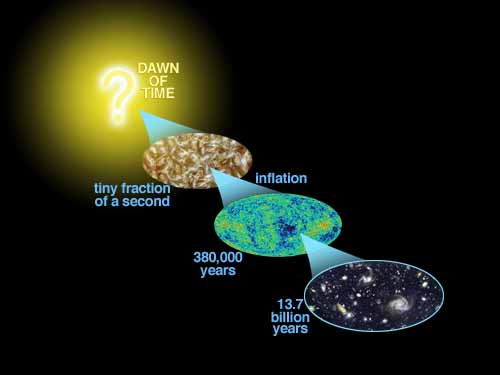
\includegraphics[width=\textwidth]{figures/wmap_cosmic_history}
\caption[Short figure name.]{ A schematic illustrating the cosmic history of structure formation from the Big Bang to today. Credit: NASA / WMAP Science Team
\label{fig:cosmic_history}}
\end{figure}

From a predominantly radiation-dominated Universe, with expansion, the density of radiation drops steeply leading to a the matter-radiation equality at ~ 50,000 years after the Big Bang. Since dark matter only interacts gravitationally, the dark matter ripples from the fluctuations form compact structures more freely as they are not opposed by other forces such as radiation pressure. Dark matter begins to collapse before ordinary matter into structures known as halos. Thus dark matter seeded the growth of structures into which baryons fell into later. Without dark matter, the age of galaxy formation would have been further delayed than as is observed in the Universe.\\

Potential refs:
Navarro Frenk White: \href{http://iopscience.iop.org/article/10.1086/304888/meta}.
Weinberg: \href{https://www.pnas.org/content/112/40/12249#ref-4}.

About 380,000 years after the Big Bang, the expansion of the Universe resulted in a lowering of density as well as a cooling down of its temperature to a point where protons and electrons in this plasma soup start combining to form the neutral hydrogen. Electrons decouple from the photons (these decoupled photons are what we detect as the CMB today) and the baryonic matter is now free to collapse under gravity creating local overdensities. We now enter the non-linear regime of structure formation where dense concentrations of matter (dark and baryonic alike) get progressively denser. Baryonic matter can additionally lose energy by radiation and can sink further into regions of high overdensity. The result of this process gives rise to a Universe that resembles a web (the cosmic web) with sheets and filaments of dark matter, creating a skeletal backbone in which star formation and galaxy formation eventually occur. The first stars and galaxies have their origins in the primordial structures that happened when the dense baryonic regions condensed within cold dark matter haloes in the cosmic web.\\

\emph{Papers to cite above?}

This abridged story of galaxy formation from fluctuations after the Big Bang to our early galaxies of course does not come close to touching upon some of the very complex phenomena involving the physics of magnetohydrodynamics, general relativity and gravitation. The interplay of these complex phenomena ... something about glaaxy simulations here...


\subsection{Galaxies as Star Formation Factories}




\subsection{Fundamental Questions in Galaxy Evolution}
{Then the questions: what ends star formation at high mass?
what  regulates it at low mass? how are 
stellar mass and DM mass related? Then finally mention
simulations that exist that compare the two, if reliable
observations can be made to compare to.}

\section{Observational Indicators of Star Formation}

Kennicutt review paper: 

{\bf MRB says: I assume this section is about observations 
of SF in galaxies. That would make sense. You need to 
introduce importance of dust here.}

{\bf MRB says: You probably want to also have something
about observation of stellar mass distribution.}

\subsection{What can we infer from Photometry?}

{\bf MRB: Maybe combine this with the next.}

\subsection{What can we infer from a Galaxy Spectrum?}

SED's: Stebbins Whitford: \href{http://adsabs.harvard.edu/abs/1968ApJ...154...21O}.

\section{Star Formation in the Local Universe}

{\bf MRB: Maybe Legacy, plus MaNGA. NSA can be mentioned
as a reanalysis of Legacy photometry}

\subsection{The Age of Digital Survey Astronomy}

\subsection{SDSS Legacy Survey}



